%!TEX root = ../../report.tex
\section{Laser range sensor}
\label{sec:laser_range_sensor}
When A. Elfes and H. Moravec introduced the occupancy grid map they also introduced the inverse sensor model, used to update a map considering the uncertainties related to measurements. 
A sensor characteristics is described with a forward sensor model, 
\begin{equation*}
	p(z|m,x)
\end{equation*}
which is the probability for measuring a distance given the location of the sensor and the obstacle the measurement hits. 
The inverse sensor model,
\begin{equation*}
	p(m|z,x)
\end{equation*}
converts these characteristics to describe the probability for occupancy of the map given the measurement. The last term in equation \vref{eq:occupancy_update} is the log-odds version of this value.

The primary sensor on mobile robot platforms used for navigation are laser range finders known as LiDar.

\subsection{Forward Sensor Model}
Laser range finders are subject to various forms of noise. In \cite{probRob} four different types of noise are combined to a model for range finders. 
The four different types of noise are:

\begin{itemize}
	\item Small Gaussian measurement noise
	\item Unexpected objects
	\item Measurement failures
	\item Random measurements
\end{itemize}

The first type of noise, the measurement noise around the correct distance, arises from small inaccuracies in the sensor and environment effects. This noise is modeled as a normal distribution and should be taken into account, when a sensor model is devised. 

The second noise type is from unexpected obstacles. This noise stems from the fact that maps represent a static image of a dynamic environment. When the robot senses the environment, it will occasionally see obstacles that are not present in the map, for instance humans moving around. These highly dynamical objects will be filtered out in the transition from static map to the dynamic map(see section ???), and thus are not a concern in the sensor model for static mapping.

The third type of noise are the measurement failures. 
For laser range finders failures can occur due to insufficient reflectance of the light on the obstacles. 
These failures often cause a maximum range reading and are handled by cutting off earlier than the maximum range.

The fourth noise type are the random measurements. This type represents entirely random readings and are modeled with a uniform distribution and should be taken into account in the sensor model.

The error on the angle which the laser points in with respect to the sensor is usually negligible \cite{probRob} \todo{Check kilde/find}.

\todo{Insert image of sensor errors, due to nearby measurements tend to have the same distance, kilde niels og forsøg}

Sebasian Thrun proposed to learn occupancy grids from the forward sensor model with expectation-maximization \cite{probRob}.
This however demands for storing a batch of measurements and is computational expensive to perform. 
It is more common to learn occupancy grids with an Inverse Sensor Model where measurements are added incrementally according to equation \vref{eq:occupancy_update}. 

\subsection{Inverse Sensor Model}
The inverse sensor model \vref{eq:occupancy_update}, describes the probability for a cell being occupied in an occupancy grid map given a sensor measurement and location.
Many different inverse sensor models have been proposed to incorporate Laser range measurements in a occupancy grid map. The individual rays are often assumed narrow and the orientation of it with respect to the robot is assumed ideal.
The simplest possible inverse sensor model is the 
ideal inverse sensor model. It assumes zero probability before the measured distance, one at the measured distance, and $0.5$ after. The model shown in figure \vref{fig:sensor_model_std_dev01} is almost ideal.

\subsubsection{Elfes Sensor Model}
R. Merali and T. Barfoot \cite{sensorModelTuning} conducted a comparison and tuning of common inverse sensor models for laser range finders in a one dimensional simulated situation. It showed that the simple model with Gaussian noise proposed by A. Elfes in \cite{elfes} performed as good using only 2 parameters, as an approximation to the complete solution with 20 parameters. They found that the model performed better, if the log odds values where limited to -12.9047. This is also used in this work.

D. Joubert derives Elfes model in \cite{Joubert2014} by convolving a Gaussian function on an ideal sensor model, describe in section \vref{sec:occupancy_grid_mapping}. While this can be done analytically, it is chosen to apply the kernel shown in figure \vref{fig:sensor_model_std_dev01} to the ideal sensor model.
The distance to the obstacle is $0.275m$ and the standard deviation of the Gaussian kernel is $1cm$. 
The maximum and minimal log-odds values are out of the scope, but they can be calculated from the probabilities with equation \vref{eq:occupancy_update}.
SICK does not indicate a standard deviation in the data-sheet for the sensor, S30B-2011, used for the MIR platform \cite{lidarDatasheet}.
According to the CTO at MIR, Niels Jul Jacobsen, a standard deviation of $1cm$ is a good approximation for the expected Gaussian noise around the read distance. 

\begin{figure}[htbp]
	\centering
	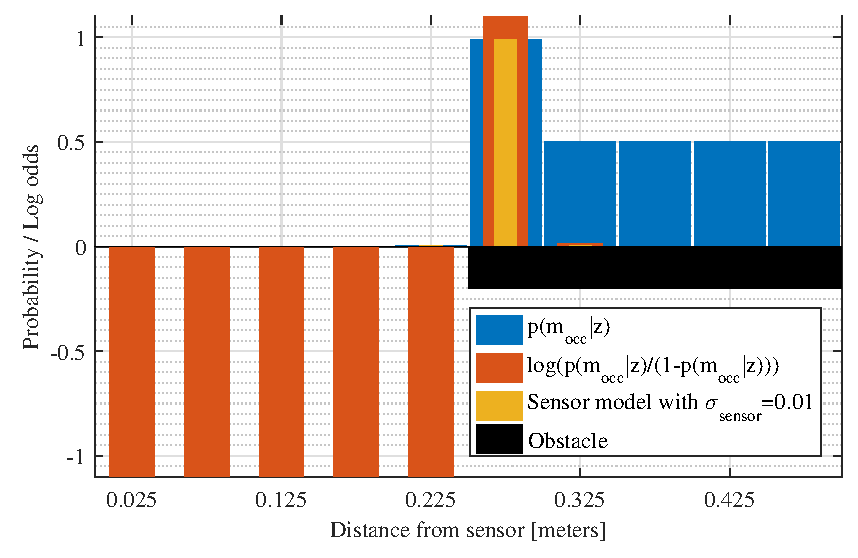
\includegraphics[scale=1.0]{figures/static_mapping/sensor_model_std_dev01}
	\caption{Elfes inverse sensor model with the expected forward sensor model.}
	\label{fig:sensor_model_std_dev01}
\end{figure}

The weights of the inverse sensor model is spread more out around the measured distance, when the standard deviation is increased, as shown in figure \vref{fig:sensor_model_std_dev025}. 
This indicates less trust in the measured distance. With this model more measurements are needed to learn the same occupancy probability, as would be achieved with the ideal model. It can however be used to avoid overconfidence in measurements while still converging to the correct map, if the measurement error is Gaussian distributed.

\begin{figure}[htbp]
	\centering
	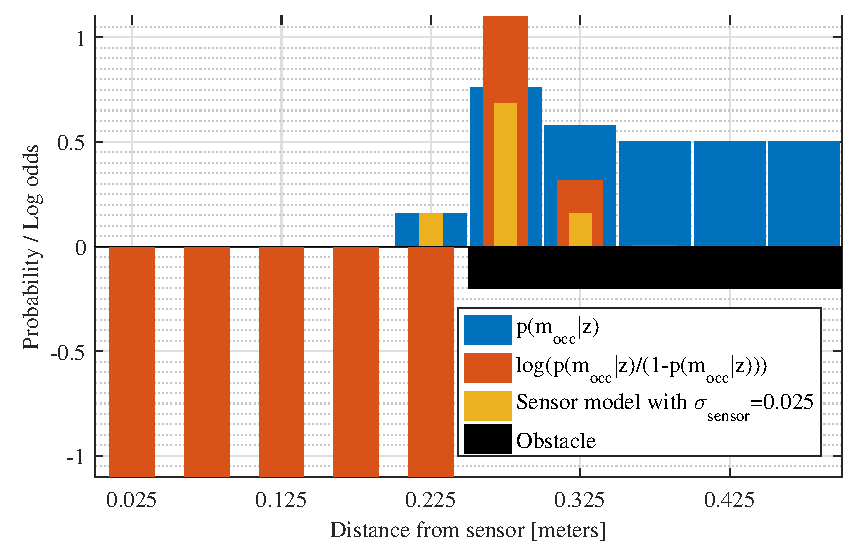
\includegraphics[scale=1.0]{figures/static_mapping/sensor_model_std_dev025}
	\caption{Elfes inverse sensor model with a larger standard deviation than that of the sensor's.}
	\label{fig:sensor_model_std_dev025}
\end{figure}

Even with the sensor noise modeled as shown in figure \vref{fig:sensor_model_std_dev01}, erroneous maps like the one shown in \vref{fig:elfes_ideal_with_poses} and \vref{fig:elfes_compare} are expected, due to localization errors.

\begin{figure}[htbp]
	\centering
	\begin{subfigure}[t]{0.45\textwidth}
		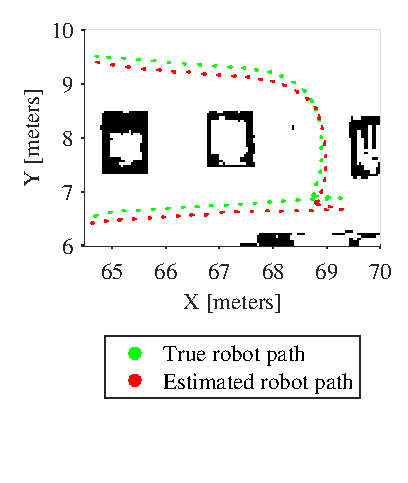
\includegraphics[scale=1.0]{figures/static_mapping/map_region_with_poses}
		\caption{Occupancy grid of the simulated world.}
		\label{fig:map_region_with_poses}
	\end{subfigure}
	\begin{subfigure}[t]{0.45\textwidth}
		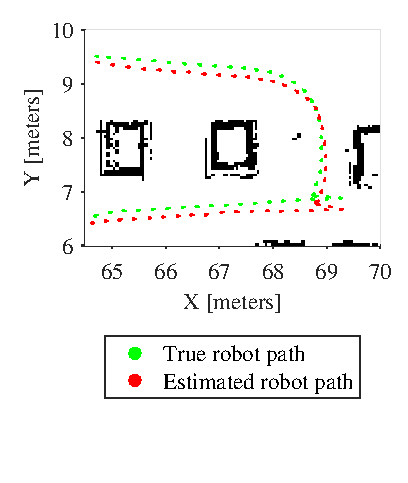
\includegraphics[scale=1.0]{figures/static_mapping/elfes_ideal_with_poses_no_decay}
		\caption{Mapped occupancy grid using the sensor model in figure \vref{fig:sensor_model_std_dev01}.}
		\label{fig:elfes_ideal_with_poses}
	\end{subfigure}
	\caption{Mapping results gained by simulating a MIR robot with imprecise location.}
	\label{fig:simulated_location_error}
\end{figure}

\begin{figure}[htbp]
	\centering
	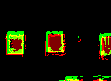
\includegraphics[width=0.5\linewidth]{figures/static_mapping/elfes_ideal_no_decay}
	\caption{Comparison between the obstacles position in figure  \vref{fig:map_region_with_poses} shown in green and the mapped obstacles in figure \vref{fig:elfes_ideal_with_poses} shown in red. The overlapping yellow regions marks areas with successful mapping.}
	\label{fig:elfes_compare}
\end{figure}

The influence of the error could be diminished by incorporating the localization errors in the inverse sensor model.
